\documentclass[12pt,a4paper]{article}
\usepackage{courier}
\usepackage{nopageno}
\usepackage[polish]{babel}
\usepackage[T1]{fontenc}
\usepackage[utf8]{inputenc}
\usepackage{amsmath,amsfonts}
\usepackage{titling}
\usepackage{mathtools}
\usepackage[margin=0.6in]{geometry} 
\usepackage{enumerate}
\usepackage{graphicx}

\title{Ćwiczenia z Sieci komputerowych \\ Zestaw 2 -- Rozwiązania}
\author{Cezary Świtała}

\begin{document}

\maketitle

\vskip 0.2cm
\noindent
\textbf{Deklaruję zadania: 1,2,3,4,5,6,7,8}
\vskip 0.2cm


\noindent
\textbf{Zadanie 1} W kablu koncentrycznym używanym w standardowym 10-Mbitowym Ethernecie sygnał rozchodzi się z prędkością \(10^8\) m/s. Standard ustala, że maksymalna odległość między dwoma komputerami może wynosić co najwyżej 2,5 km. Oblicz, jaka jest minimalna długość ramki (wraz z nagłówkami.

\vskip5pt
\noindent
\textbf{Rozwiązanie:}
Czas propagacji wynosi 
\[ 2500 \div 10^8 = 0,000025s.\]
Chcemy, żeby czas wysyłania był dłuższy niż dwukrotność czasu propagacji, zatem większy niż \(0,00005s\). Przesyłamy \(10^7\) bitów na sekundę, zatem rozmiar ramki musi być większy niż 

\[
10^7 \cdot 0.00005s = 500
\]
bitów, czyli dłuższy niż 63 bajty.

\vskip10pt

\noindent
\textbf{Zadanie 2} Rozważmy rundowy protokół Aloha we współdzielonym kanale, tj. w każdej rundzie każdy z \(n\) uczestników usiłuje wysłać ramkę z prawdopodobieństwem \(p\). Jakie jest prawdopodobieństwo \(P(p,n)\), że jednej stacji uda się nadać (tj. że nie wystąpi kolizja)? Pokaż, że \(P(p,n)\) jest maksymalizowane dla \(p=1/n\). Ile wynosi \(lim_{n \rightarrow \infty} P(1/n, n)\)?

\vskip5pt

\noindent
\textbf{Rozwiązanie:} Prawdopodobieństwo na to, że k-temu komputerowi uda się nadać to \(p(1-p)^{n-1}\). Zatem

\[
P(p,n) = \sum_{k=1}^{n} p(1-p)^{n-1} = np(1-p)^{n-1}.
\]
Żeby wyznaczyć maksima należy spojrzeć na miejsca zerowe pierwszej pochodnej.

\begin{gather*}
P'(p,n) = n(1-p)^{n-1} - np(n-1)(1-p)^{n-2} = \\
= n(1-p)^{n-2}( 1 - p - np + p ) = \\
= n(1-p)^{n-2}( 1 - np )
\end{gather*}
\newpage
\noindent
Dwa miejsca zerowe: \(p = 1\), \(p = 1/n\). Monotoniczność można odczytać z rysunku:

\begin{center}
	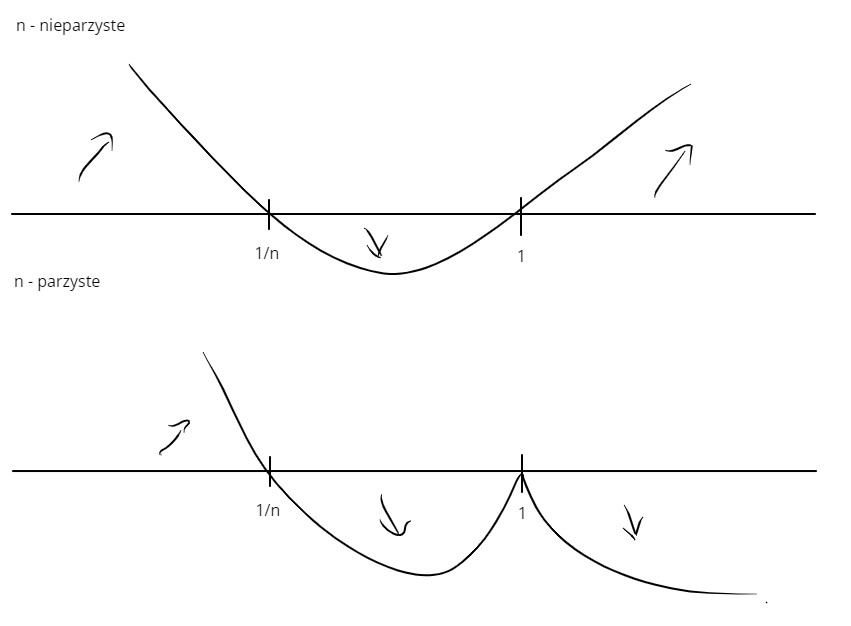
\includegraphics[scale=0.5]{mon.jpg}
\end{center}
Rozważamy \(p\) w zakresie od 0 do 1, zatem maksimum mamy dla \(p=1/n\). Następnie policzyć trzeba \(lim_{n \rightarrow \infty} P(1/n, n)\).
\[
 lim_{n \rightarrow \infty} P(1/n, n) = lim_{n \rightarrow \infty} n \cdot \frac{1}{n} \left( 1-\frac{1}{n} \right) ^{n - 1} = \frac{1}{e}
\]

\vskip10pt

\noindent
\textbf{Zadanie 3} Wyszukaj w sieci informację na temat zjawiska \emph{Ethernet capture} i wytłumacz w jaki sposób ono powstaje. (Ty mianem określa się sytuację, w której jedna ze stacji nadaje znacznie częściej, choć wszystkie stacje używają algorytmu CSMA/CD.)

\vskip5pt
\noindent
\textbf{Rozwiązanie:} Zjawisko ma miejsce kiedy jedna ze stacji przesyła dużą ilość danych i przejmuje łącze na kilkanaście kolejnych rund, gdyż z każdym wygranym konfliktem ma większą szansę na wygranie kolejnego.

Na przykład jeśli mamy łącze na którym nadawać chce jednocześnie \(A\) i \(B\) to powstanie konflikt, oba nadajniki wylosują time-out ze zbioru \(\{0, 2^1-1\}\). Załóżmy, że wygrał \(A\) i nadał swój pierwszy pakiet. Przy próbie nadania drugiego znów wystąpi konflikt, dla \(B\) będzie to druga porażka, zatem wylosuje time-out ze zbioru \(\{0,...,2^2-1\}\), dla \(A\) to pierwszy konflikt na tym pakiecie, dlatego znów wylosuje time-out z \(\{0,1\}\). \(A\) ma większe prawdopodobieństwo wygranej i z każdą kolejną wygraną próbą będzie miał większe szanse na wygranie kolejnej. W praktyce często się zdarza, że \(A\) wygrywa wszystkie konflikty, aż \(B\) się nie podda i przejdzie do wysyłania kolejnej ramki.

Mimo, że tworzy to niesprawiedliwość w przydziale czasu nadawania, to jest ona łagodzona przez fakt, że każdy nadajnik ma szansę przejąć łącze co jakiś czas. Poza tym zjawisko to ma największe szanse wystąpienia na łączach z niewielką liczbą nadajników.

\vskip10pt
\noindent
\textbf{Zadanie 4} Jaka suma kontrolna CRC zostanie dołączona do wiadomości 1010 przy założeniu, że CRC używa wielomianu \(x^2 + x + 1\)? A jaka jeśli używa wielomianu \( x^7 + 1 \)?

\vskip5pt
\noindent
\textbf{Rozwiązanie:} Używamy \(G(x) = x^2 + x + 1\), czyli suma CRC będzie mieć 2 bity. Wiadomość \(M(x) = x^3 + x\) przemnożona o \(x^2\) i zwiększona o sumę \(S(x)\) musi być podzielna przez \(G(x)\), czyli chcemy

\[
 G(x)~ |~ M(x) x^2 + S(x)
\]
Wystarczy dobrać \(S(x)\) tak żeby wyzerowało resztę z dzielenia, a ponieważ działamy w \(\mathbb{F}_2\) wystarczy że będzie równe reszcie z dzielenia.

\[
	S(x) = M(x)x^2 \mod G(x) = x
\]
\(S(x)\) kodujemy binarnie jako \texttt{10}.

Jeśli użyjemy \(G(x) = x^7 + 1\) to suma CRC będzie mieć 7 bitów. Postępujemy analogicznie i dostaniemy
\[
	S(x) = M(x)x^7 \mod G(x) = 	x^3 + x
\]
\(S(x)\) kodujemy binarnie jako \texttt{0001010}.

\vskip10pt

\noindent
\textbf{Zadanie 5} Pokaż, że CRC-1, czyli 1-bitowa suma obliczana na podstawie wielomianu \(G(x) = x + 1\), działa identycznie jak bit parzystości.
\vskip5pt
\noindent
\textbf{Rozwiązanie:} Chcemy pokazać że jedno bitowa suma kontrolna CRC-1 będzie zachowywać się tak samo jak bit parzystości, tzn. będzie jedynką jeśli liczba zapalonych bitów będzie nieparzysta, a zerem wpp.

Można skorzystać z twierdzenia Bezouta, które mówi, że jeśli \(\mathbb{F}\) jest ciałem, \(\mathbb{F}{[x]}\) pierścieniem wielomianów o współczynnikach z tego ciała, zaś \(f,(x-c) \in \mathbb{F}[x]\) wielomianami z tego pierścienia, to reszta z dzielenia \(f\) przez \((x-c)\) to \(f(c)\).

W naszym przypadku dzielimy przez \(x+1\), zatem \(c = 1\). Resztą z dzielenia, a co za tym idzie sumą kontrolną, będzie zatem wartość wielomianu \(M(x)x\) w punkcie \(1\). Jeśli wielomian ten miał parzystą liczbę niezerowych współczynników to wynikiem będzie 0, wpp. 1, czyli suma zachowuje się jak bit parzystości.

\vskip10pt
\noindent
\textbf{Zadanie 6} Załóżmy, że wielomian \(G(x)\) stopnia \(n\) stosowany w CRC zawiera składnik \(x^0\). Pokaż, że jeśli wybierzemy dowolny odcinek długości \(n\) z wiadomości i dowolnie go zmodyfikujemy (zmienimy dowolną niezerową liczbę bitów w nim), to zostanie to wykryte. Czy taka własność zachodzi, jeśli \(G(x)\) nie zawiera składnika równego \(x^0\)?

\vskip5pt
\noindent
\textbf{Rozwiązanie:} Dowolne przekłamanie ciągu bitów długości nie większej niż \(n\) bitów to inaczej dodanie do oryginalnej wiadomości jakiegoś wielomianu \(E(x)\). Jeśli \(j\) jest pozycją ostatniego przekłamanego bitu, to
\[
	E(x) = x^je(x),
\]
gdzie \(e(x)\) to wielomian stopnia mniejszego niż \(n\). Zmiana zostanie wykryta jeśli po dodaniu do oryginalnej wiadomości (podzielnej przez \(G\)) wielomianu \(E(x)\), wiadomość stanie się niepodzielna. Czyli chcemy pokazać że \(G(x) \not|~ E(x)\). \(G(x)\) jest względnie pierwsze z \(x^j\), bo ma składnik \(x^0\), zatem wystarczy pokazać, że nie dzieli \(e(x)\).

Zauważmy, że 
\[
	deg(G) > deg(e),
\]
zatem resztą z dzielenia \(e(x)\) przez \(G(x)\) jest dokładnie \(e(x)\), a jest ono niezerowe, czyli \(G(x)\) nie dzieli też \(E(x)\), więc błąd zostanie wykryty. 

Własność nie musiałaby zajść, gdyby \(G(x)\) nie miało składnika \(x^0\), gdyż wtedy nie mielibyśmy względnej pierwszości. Np weźmy \(G(x) = x\) i jakąś poprawną wiadomość z sumą kontrolną. Jeśli dokonamy przekłamania drugiego bitu \(E(x) = x\) to nie wykryjemy tej zmiany bo podzielność się nie zmieni. 



\vskip10pt

\noindent
\textbf{Zadanie 7} Pokaż, że kodowanie Hamming(7,4) umożliwia skorygowanie jednego przekłamanego bitu. Wskazówka: wystarczy pokazać, że odległość Hamminga między dwoma kodami wynosi co najmniej 3.
\vskip5pt
\noindent
\textbf{Rozwiązanie:} W kodowaniu Hamming(7,4) przeplatamy bity parzystości \(p_1,p_2,p_4\) z bitami danych \(d_3, d_5, d_6, d_7\) tworząc wektor \([ p_1, p_2, d_3, p_4, d_5, d_6, d_7 ]\). Bit \(p_1\) jest bitem parzystości dla trójki bitów \(d_3, d_5, d_7\), bit \(p_2\) dla \(d_3, d_6, d_7\), a bit \(p_4\) dla \(d_5, d_6, d_7\). W ogólności \(p_i\) jest bitem parzystości dla bitu \(d_x\) jeśli x ma jedynkę na \(log_2(i)+1\)-tym bitcie od prawej. Chcemy pokazać, że dowolne dwa poprawne kody różnią się co najmniej na trzech bitach.

\vskip5pt

\noindent
Obserwacja 1: Istnieje 16 poprawnych kodów, po jednym dla każdej możliwej wartości bitów danych.

\noindent
Obserwacja 2: Każdy z bitów \(d_3, d_5, d_6, d_7\) ma wpływ na co najmniej 2 bity parzystości.

\noindent
Obserwacja 3: Żadne dwa różne bity spośród \(d_3,d_5,d_6\) nie wpływają na dwa te same bity parzystości. Bit \(d_7\) ma wpływ na trzy bity parzystości.

\vskip5pt

Weźmy dowolne dwa różne poprawne kody. Muszą one różnić się na bitach danych. Interesujące są tylko przypadki, w których różnią się na mniej niż trzech miejscach, więc albo dokładnie na jednym, albo dokładnie na dwóch (bo wpp mamy tezę za darmo).

\begin{enumerate}
	\item Jeśli różnią się w dokładnie jednym miejscu, to z obserwacji 2 wynika, że kody muszą różnić się też na co najmniej dwóch bitach parzystości.
	\item Jeśli różnią się na dwóch bitach danych i żadnym z nich nie jest \(d_7\), to wiemy że co najmniej jeden bit parzystości (jeden z tych na które oba nie mają wpływu), też musi być inny.
	\item Jeśli różnią się na dwóch bitach danych \(d_i, d_7\) to różnić się będą też na bitcie parzystości na który nie miało wpływu \(d_i\), gdyż \(d_7\) ma wpływ na wszystkie trzy.
\end{enumerate}
W każdym przypadku kody różnią się co najmniej 3 bitami.

\vskip10pt
\noindent
\textbf{Zadanie 8} Pokaż, że suma CRC stosująca wielomian \(G(x) = x^3 + x + 1\) wykryje wszystkie podwójne błędy (zmianę wartości dwóch bitów), które są oddalone od siebie o nie więcej niż 6 bitów (tj. pomiędzy dwoma zmienianymi bitami jest nie więcej niż 5 innych bitów).

\vskip5pt
\noindent
\textbf{Rozwiązanie:} Przekłamanie dwóch bitów oddalonych o mniej niż 6 bitów to inaczej dodanie do oryginalnej wiadomości jakiegoś wielomianu \(E(x)\). Jeśli \(j\) jest pozycją ostatniego przekłamanego bitu, to

\[
	E(x) = x^je(x),
\]
gdzie \(e(x)\) to wielomian w postaci \(x^n + 1\), stopnia mniejszego lub równego 6.
Chcemy pokazać, że po dodaniu \(E(x)\), \(G(x)\) nie podzieli wiadomości, czyli że \( G(x) \not|~ E(x)\).

\(G(x)\) jest względnie pierwsze z \(x^j\), zatem wystarczy pokazać, że \(G(x)\) nie dzieli \(e(x)\). Można sprawdzić każdy możliwy stopień tego wielomianu.

\begin{enumerate}
	\item Dla \(n \in \{1,2\}\) wielomian jest niepodzielny przez \(G(x)\), bo ma mniejszy stopień.
	\item Dla \(n = 3\) reszta \(x\).
	\item Dla \(n = 4\) reszta \(x^2 + x\)
	\item Dla \(n = 5\) reszta \(x^2 + x\)
	\item Dla \(n = 6\) reszta \(x\)
\end{enumerate}
W każdym przypadku dostajemy resztę zatem zmodyfikowanie dwóch bitów zostałoby wykryte.


\end{document}
